\documentclass[a4paper, 11pt]{article}

% Nécessaire
\usepackage[french]{babel}
\usepackage[utf8]{inputenc}
\usepackage[T1]{fontenc}
\usepackage{lmodern}
\usepackage{amsmath, amsthm}
\usepackage{amsfonts,amssymb}

% Marge
\usepackage{geometry}
\geometry{margin={2.2cm ,2cm}}

% Figures, graphiques
\usepackage{graphicx}
\usepackage{epsfig}
\usepackage{caption}

% Surlignage
\usepackage{alltt}

\usepackage{xcolor}
\usepackage{soul}
\usepackage{color}
\usepackage{colortbl}

% Indicatrice
\usepackage{dsfont}

\usepackage{multirow}
\usepackage{eurosym}
\usepackage{extarrows}

% Graphique
\usepackage{tikz}


% Titre
\title{Modèle}
\author{}
\date{}



\begin{document}
\maketitle  

Le manguier est un arbre qui présente de forts asynchronismes inter- et intra-arbres. Cette particularité induit une fenêtre d'exposition élargie des inflorescences et des fruits aux ravageurs. Parmi ceux-ci se trouve la cécidomyie qui pond dans les inflorescences, pouvant provoquer la mort de celles-ci.

\section{Connaissances}

\subsection{Inflorescences des manguiers}

Les inflorescences ont une durée de vie théorique de 50 jours. Au cours de son développement, l'inflorescence traverse plusieurs stades phénologiques : C/D, E, F/PF. Ce que l'on considère comme la naissance est en fait le débourrement qui marque également le début du stade C. Les durées des différents stades phénologiques sont les suivantes :
\begin{itemize}
 \item C/D : 7 jours;
 \item E : 9 jours;
 \item F/PF : 34 jours.
\end{itemize}
Ces stades influent probablement sur l'attractivité des inflorescences sur les cécidomyies.

\subsection{Cécidomyies}

\begin{figure}[ht]
 \centering
 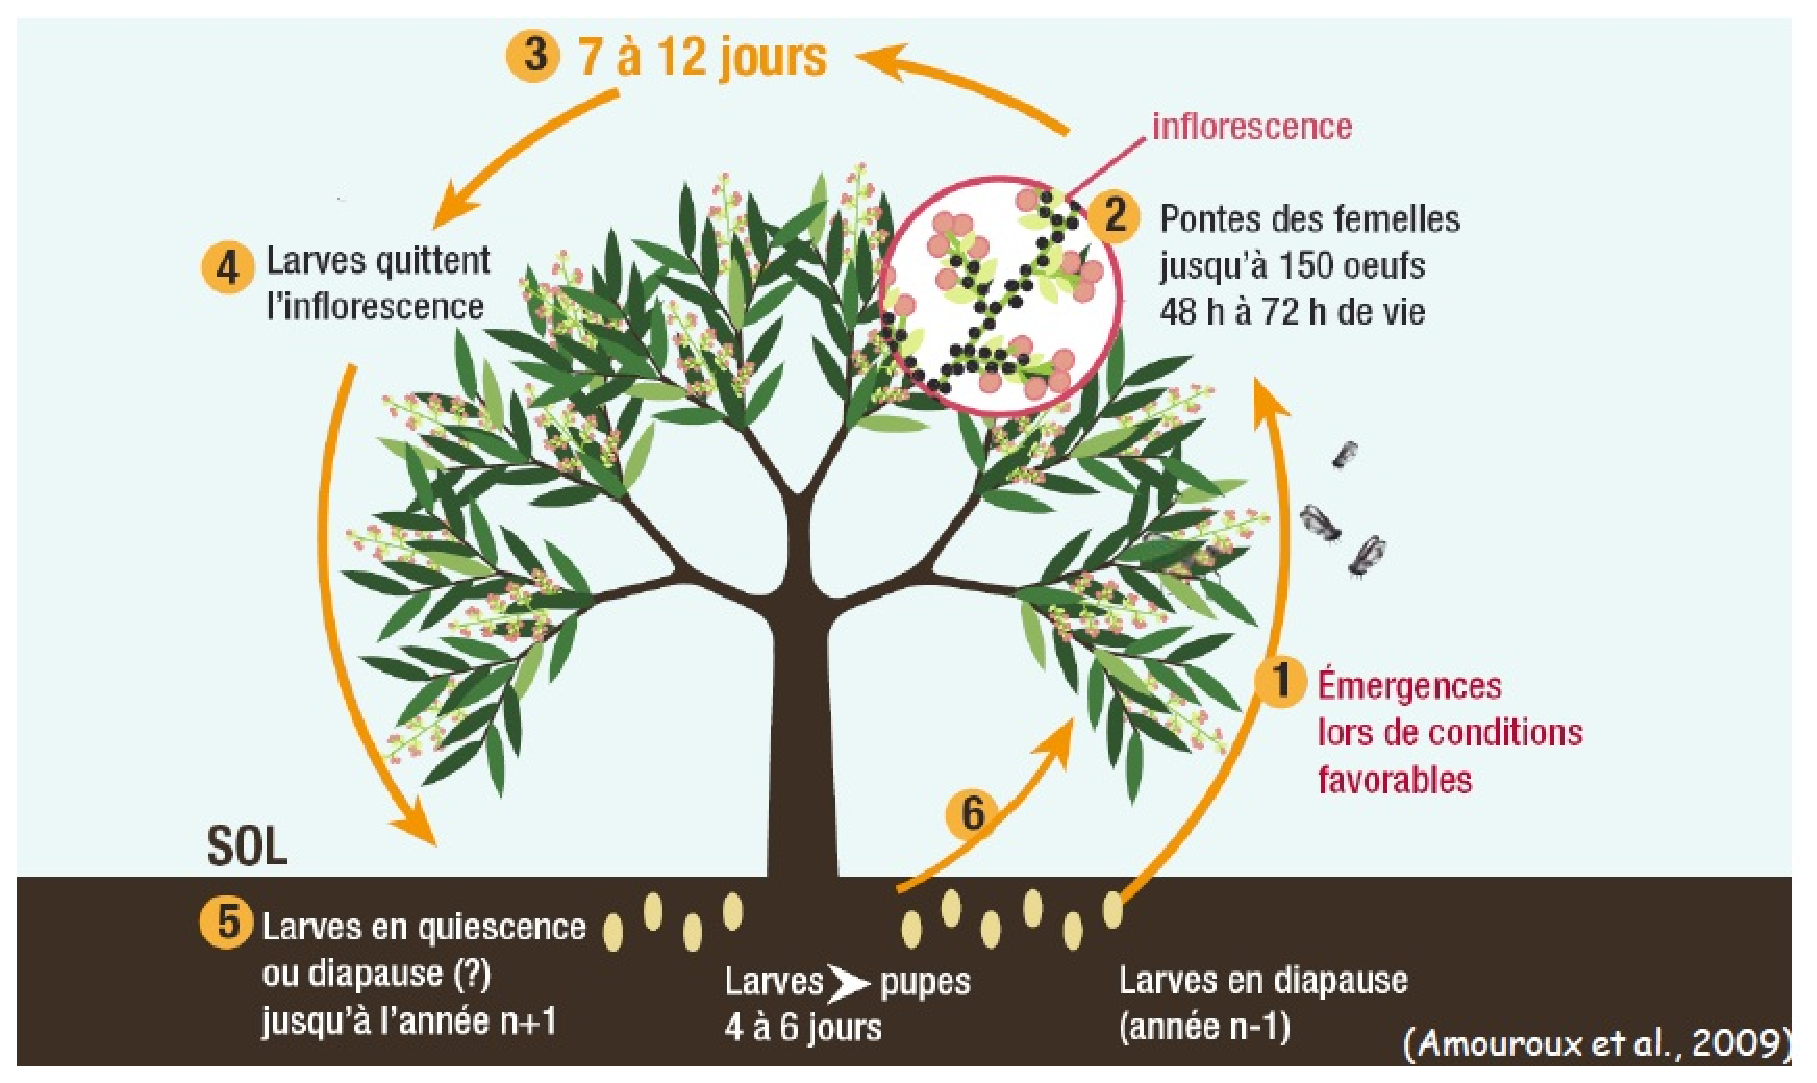
\epsfig{file = plots/cycle.eps, scale = 0.4}
 % cycle.png: 856x504 px, 96dpi, 22.65x13.34 cm, bb=0 0 642 378
 \caption{Cycle de développement des cécidomyies}
 \label{fig:cycle}
\end{figure}

Le cycle de développement des cécidomyies est présenté sur la figure~\ref{fig:cycle}. Les femelles présentes dans le verger à la date $t$ pondent des œufs dans les inflorescences. Sept à douze jours plus tard, les œufs se sont transformés en larves et s'éjectent des inflorescences pour aller s'enfouir dans le sol. Dans le sol, les larves peuvent soit entrer en diapause, soit entrer en pupaison. Si elles entrent en diapause, alors les femelles ne ressortent que l'année suivante. Si elles entrent en pupaison, alors le cycle de développement se poursuit et des cécidomyies adultes émergent quatre à six jours plus tard, perpétuant ainsi le cycle.

\section{Données}

Une expérimentation a été faite en 2017 et 2018 pour tester un éventuel effet de la modalité de couverture du sol sur l'impact des cécidomyies. Un verger a été séparé en trois, chacune des parties ayant une modalité de couverture du sol différente : enherbement ras, paillage synthétique ou enherbement haut.

Pour l'année 2017 on dispose de deux suivis sur ce verger, donnant deux jeux de données.
Le \textit{dataset 1} porte sur les inflorescences : leurs dates de débourrements et leurs dates de morts sont recensées.
Cela nous permet d'avoir le nombre d'inflorescences vivantes à chaque date, mais aussi la durée de vie moyenne observée d'une inflorescence ainsi que des estimations de la proportion des différents stades phénologiques des inflorescences à chaque date.

Le \textit{dataset 2} porte sur les cécidomyies et les inflorescences. Des pièges ont été placés sous les inflorescences pour récolter les larves qui s'en éjectent dans chacun des trois sous-vergers. On a le nombre d'inflorescences vivantes au-dessus des pièges et le nombre des inflorescences des arbres suivis et le nombre de larves piégées à chaque date.

En se basant sur le \textit{dataset 2}, il a également été possible de reproduire la dynamique d'inflorescences vivantes, en la simulant. Cela nous permettra de créer des dynamiques dites attractives.

\begin{figure}[ht]
\centering
 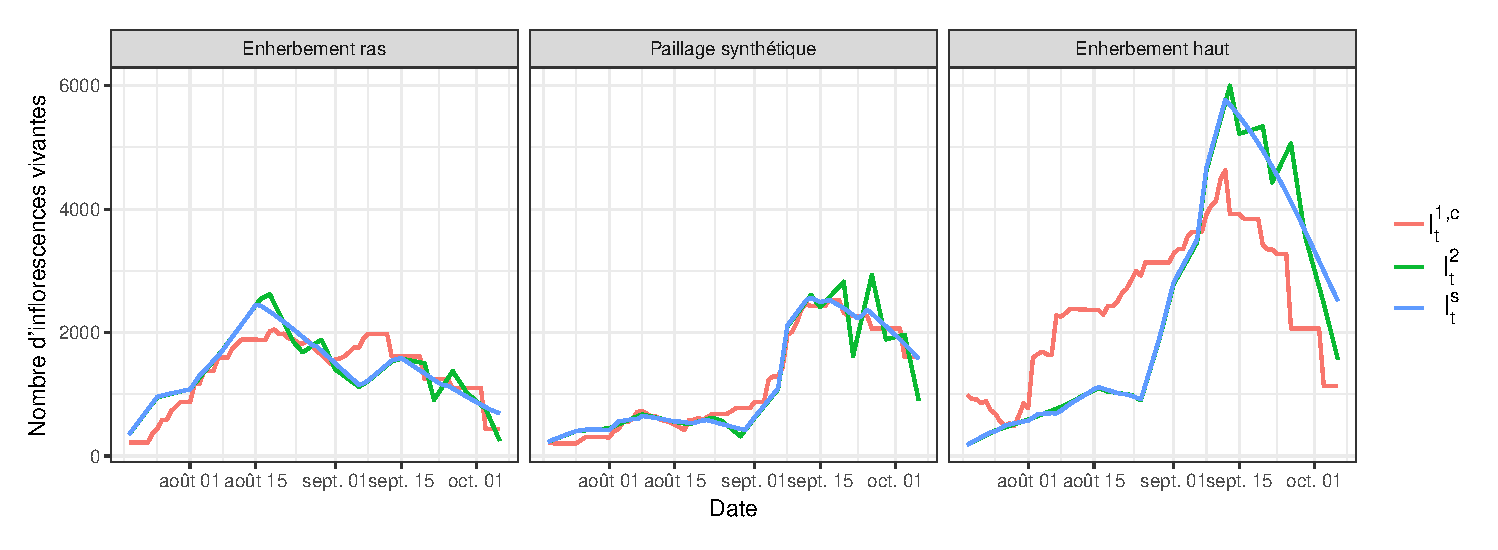
\epsfig{file = plots/comp_dyn.eps, scale = 0.67}
 \caption{Comparaison des trois dynamiques d'inflorescences obtenues : $I_t^{1, c}$ est issue du \textit{dataset 1}, $I_t^2$ est issue du \textit{dataset 2} et $I_t^s$ est simulée.}
 \label{fig:comp}
\end{figure}



\section{Hypothèses}

Pour modéliser le phénomène, on émet des hypothèses.

\begin{itemize}
 \item \textbf{Les femelles ne vivent qu'un jour :} les femelles pondent et meurent le jour de leur émergence ou de leur venue dans le verger;
 \item \textbf{aucune cécidomyie n'émerge du sous-bloc baché :} les larves ne peuvent s'enfouir dans le sol lorsque qu'une bache est présente, les individus en diapause ne peuvent pas émerger lorsqu'une bache est présente;
 \item \textbf{les femelles exogènes viennent proportionnellement aux inflorescences présentes};
 \item \textbf{les individus en diapause sont confondus avec les individus exogènes :} il n'est (pour l'instant) pas possible de faire la distinction entre les individus qui émergent de diapause et ceux qui arrivent de l'extérieur ;
 \item \textbf{il y a des échanges de femelles entre les trois sous-blocs :} on considère cependant que les femelles préfèrent rester dans le sous-bloc duquel elles émergent. Si elles quittent le sous-blocs, elles s'en vont dans le sous-bloc limitrophe (le sous-bloc baché, en l'occurrence);
 \item \textbf{les manguiers ne sont pas impactés par la modalité de couverture du sol, le vol des cécidomyies non plus :} on considère que la modalité de couverture du sol n'impacte que la survie des individus lorsqu'il s'enfouissent dans le sol puis quand ils en émergent.
\end{itemize}


\section{Modèle}

Les phénomènes et hypothèses susmentionnés sont modélisés par des équations. Ainsi, le nombre de larves qui s'éjectent des inflorescences dans le sous-bloc $i$ le jour $t$ est déterminé par
$$L_{t, i} = N_{t-d_\ell, i} \times R \times E_0 \times \mu_\ell,$$
où $N_{t-d_\ell, i}$ représente le nombre de femelles présentes dans le sous-bloc $i$ une durée de larvation auparavant, $R$ le coefficient de disponibilité en ressources, $E_0$ le nombre d'œufs pondus par une femelle et $\mu_\ell$ la probabilité de survie des œufs. Et on a $R = \max\left( 1, k I_{t, i} / N_{t, i} \right)$, avec le coefficient $k$ à déterminer.

Le nombre de femelles émergeantes du sous-bloc $i$ au jour $t$ est donnée par
$$N^{\text{emer}}_{t, i} = L_{t - d_p, i} \times p_p \times \mu_p \times \mu_{\text{sol}} \times \frac{1}{1+SR},$$
avec $L_{t - d_p, i}$ le nombre de larves présentes une durée de pupaison auparavant, $p_p$ la probabilité pour une larve d'entrer en pupaison, $\mu_p$ la probabilité de survivre à la phase de pupaison, $\mu_{\text{sol}}$ la probabilité de survivre à la couverture du sol et $SR$ le \textit{sex-ratio}.

La population de femelles dans le sous-bloc $i$ au jour $t$ est donnée par
$$
N_{t, i} = N^{\text{endo}}_{t, i} + N^{\text{exo}}_{t, i}  + N^{\text{side}}_{t, i},
$$
où $N^{\text{endo}}_{t, i}$ représente le nombre de femelles émergentes du sous-bloc $i$ au jour $t$ et qui y restent, $N^{\text{exo}}_{t, i}$ le nombre de femelles exogènes au bloc venant dans le sous-bloc $i$ le jour $t$ et $N^{\text{side}}_{t, i}$ le nombre de femelles ayant émergées dans le(s) sous-bloc(s) $j$ et/ou $k$ le jour $t$ et venant dans le sous-bloc $i$.
Plus précisément, on a 
$$
N^{\text{exo}}_{t, i} = \gamma \times I_{t, i}
$$
(avec $\gamma$ à déterminer),
$$
 N^{\text{endo}}_{t, i} = \left(\frac{I_{t, i}}{I_{t, i} + I_{t, \text{lim}}} + \left( 1-p_m \right)\frac{I_{t, \text{lim}}}{I_{t, i} + I_{t, \text{lim}}}\right) N^{\text{emer}}_{t, i}, 
$$
avec $I_{t, \text{lim}}$ et $N_{t, \text{lim}}$ désignant respectivement le total des inflorescences et des femelles présentes dans le(s) sous-bloc(s) limitrophe(s), et  $p_m$ est à déterminer. Enfin
$$
N^{\text{side}}_{t, i} = p_m \frac{I_{t, j}}{I_{t, i} + I_{t, j}} N^{\text{emer}}_{t, j} \mathbf{1}_{\text{lim}(i, j)} +p_m \frac{I_{t, k}}{I_{t, i} + I_{t, k}} N^{\text{emer}}_{t, k} \mathbf{1}_{\text{lim}(i, k)},
$$
où $\mathbf{1}_{\text{lim}(i, j)}$ vaut 1 si les sous-blocs $i$ et $j$ sont limitrophes, et 0 sinon.


\end{document}

